\documentclass[a4paper,12pt]{memoir}
\usepackage{msiu_term_work}

\lstset{language=Ruby,inputencoding=utf8/koi8-r,basicstyle=\small,
stringstyle=\ttfamily,xleftmargin=1cm}

\begin{document}
\renewcommand{\contentsname}{{\Large{Оглавление}\hfill}}

\title{Методы хранения и обработки информации}
{Вычисляется сумма углов, пол которыми рёбра выпуклой оболочки пересекают заданную прямую.Вычисляет сумму площедей граней, все вершины которых-хорошие точки.}
{2362}
{А.\+Ю.~Дьячук}
{к.ф.-м.н., доцент}
{Е.\+А.~Роганов}
{2012}

\section{Введение}

В данной курсовой работе рассматриваются модификации двух эталонных проектов <<Выпуклая оболочка>> и <<Изображение проекции полиэдра>>, реализованных на объектно-ориентированном языке программирования высокого уровня Ruby.

Целями работы являются:
\begin{itemize}
\item в проект <<Выпуклая оболочка>> добавить вычисление суммы внутренних углов выпуклой оболочки;
\item <<научить>> программу определять и выводить сумму углов, под которыми рёбра выпуклой оболочки пересекают заданную прямую в проекте <<Выпуклая оболочка>>;
\item добавить в проект <<Изображение проекции полиэдра>> вывод суммы площадей граней, все вершины которые расположены вне сферы $x^2+y^2+z^2=1$.
\end{itemize}

Для того чтобы выполнить полученные задания, необходимо было изучить особенности языка Ruby, подробно разобрать каждый эталонный проект и применить полученные знания в области информатики, компьютерной математики и аналитической геометрии на плоскости и в пространстве.

\endinput


\section{Модификация проекта <<Выпуклая оболочка>>}

\subsection{Постановка задачи}

Модифицируйте эталонный проект таким образом, чтобы вычислять сумму углов, под которыми рёбра выпуклой оболочки пересекаю заданную прямую.


\subsection{Решение}

После запуска программа предлагает пользователю ввести последовательно координаты вершин выпуклой оболочки. Введённая точка индуктивно добавляется в выпуклую оболочку. Нам же необходимо вместе со значениями периметра и площади выпуклой оболочки выводить сумму острых внутренних углов.
Это задание не требует серьёзной модификации исходного кода, все функции будут вписываться в файл проекта \verb|convex.rb|.

Для выполнения задания необходимо вычислять внутренние углы, используя координаты вершин выпуклой оболочки. В языке Ruby имеется особый механизм множественного наследования \verb|(mixin)| \verb|Math|, которая содержит методы вычисления простейших тригонометрических функций, в частности, в данном проекте используется \verb|Math.acos|.

Из аналитический геометрии извеcтно, что угол между векторами $\overline{BA}$ и $\overline{BC}$ можно найти по формуле 
$$\cos(B) =\dfrac{\overline{BA}\cdot \overline{BC}}{|\overline{BA}|\cdot|\overline{BC}|}.$$

Для точек $A(X_1;Y_1)$ и $B(X_2;Y_2)$ координаты вектора $${AB}=\{X_2-X_1;Y_2-Y_1\}.$$
Если $\overline{BA}\{X_1;Y_1\}$ и $\overline{BC}\{X_2;Y_2\}$, то скалярное произведение этих векторов
$$\overline{BA}\cdot \overline{BC}=X_1X_2+Y_1Y_2,$$ а длина вектора $$\sqrt{\overline{BA}^2}=|\overline{BA}|=\sqrt{X_1^2+Y_1^2}.$$

Окончательная формула для угла B между векторами $\overline{BA}$ и $\overline{BC}$ выглядит так:
$$\cos(B) =\dfrac{X_1X_2+Y_1Y_2}{\sqrt{X_1^2+Y_1^2}\cdot\sqrt{X_2^2+Y_2^2}}.$$

Метод \verb|Math.acos| возвращает угол в радианах. Так как решено выводить ответ в градусах, воспользуемся формулой $\alpha^\circ = \alpha \times \frac{180}{\pi}$.

\subsection{Модификация кода}



Метод, который находит уравнение прямой, заданной двумя точками:

\begin{small}
\begin{verbatim}
  def equation_from_segment(p1, p2)
 
    # Ax + By + C = 0
    x1, y1 = p1.x, p1.y
    x2, y2 = p2.x, p2.y

    a = y1 - y2
    b = x2 - x1
    c = x1 * y2 - x2 * y1
    [a, b, c]
  end
\end{verbatim}
\end{small}


Метод, который находит точку пересечения линия $AB$ и отрезка $PQ$:

\begin{small}
\begin{verbatim}
  def cross_point(a, b, p, q)
    a1, b1, c1 = equation_from_segment(a, b)
    a2, b2, c2 = equation_from_segment(p, q)
    d = (a1*b2-a2*b1)
    
    # Если прямые не перескаются - завершаем работу:
    # отрезки тоже не будут пересекаться:
    return false if d == 0

    # Находим координаты пересечения прямых:
    x = -(c1*b2-c2*b1).to_f / d
    y = -(a1*c2-a2*c1).to_f / d

    # Точка пересечения прямых должна принадлежать отрезку PQ:
    m = R2Point.new(x, y)
    return false unless m.inside?(p, q)
    m
  end 
\end{verbatim}
\end{small}

Метод нахождения угла $B$:

\begin{small}
\begin{verbatim}
  def angle (a, b, c)
    
    # Координаты векторов:
    ba_x = a.x - b.x
    ba_y = a.y - b.y
    bc_x = c.x - b.x
    bc_y = c.y - b.y

    dot_product = ba_x*bc_x + ba_y*bc_y 
    module_ba = ba_x**2 + ba_y**2
    module_bc = bc_x**2 + bc_y**2
    cos = dot_product / Math.sqrt(module_ba * module_bc)
    cos *= -1 if cos < 0
	    return Math.acos(cos)
  end
\end{verbatim}
\end{small}


Увидеть работу этой модификации можно на рис.~1.

\begin{figure}[ht!]
\begin{center}
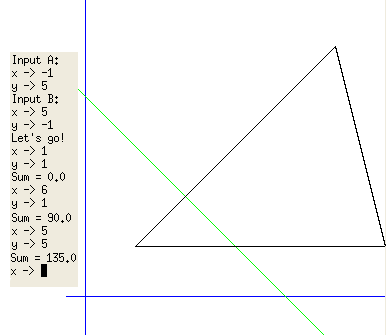
\includegraphics[scale=0.6]{images/111}
\end{center}
\vspace*{-8mm}
\caption{Вычисление суммы углов, под которыми рёбра выпуклой оболочки пересекают заданную прямую}\label{fig:term_1}
\end{figure}

\section{Модификация проекта <<Изображение проекции полиэдра>>}

\subsection{Постановка задачи}

Модифицируйте эталонный проект таким образом, чтобы определялась и печаталась следующая характеристика полиэдра: сумма площадей граней, все вершины которые расположены вне сферы.

После запуска программы, программа вычисляет площадь полигонов, которые расположены вне сферы.
Это задание не требует серьёзной модификации исходного кода, все функции будут вписываться в файл проекта \verb|polyedr.rb|.

\subsection{Решение}

Для выполнения задания необходимо определить хорошую точку в пространстве,если она строго находится вне сферы $x^2+y^2+z^2=1$.  Вычислить сумму площадей граней, все вершины которые расположены вне сферы $x^2+y^2+z^2=1$.



\subsection{Модификация кода}

Создадим метод модуля.

\begin{small}
\begin{verbatim}
 def length
    Math.sqrt(@x*@x + @y*@y + @z*@z)
 end
\end{verbatim}
\end{small}

Метод, который вычисляет вершины, который лежат вне сферы $x^2+y^2+z^2=1$:

\begin{small}
\begin{verbatim}
 def good?
    @x*@x + @y*@y + @z*@z > 1#
 end
\end{verbatim}
\end{small}


Метод, который вычисляет площадь грани:

\begin{small}
\begin{verbatim}
 def area
    result = 0.0

    for i in 1 ... (vertexes.size - 1)
      result += triangle_area(vertexes[0], vertexes[i], vertexes[i + 1])
    end

    return 0.5*result
 end 
\end{verbatim}
\end{small}

Метод, который вычисляет сумму площадей треугольников:

\begin{small}
\begin{verbatim}
 def triangle_area(a, b, c)
    ((b - a).v(c - a)).length
 end
\end{verbatim}
\end{small}

Метод который вычисляет площадь грани, если она расположена вне сферы:

\begin{small}
\begin{verbatim}
 def good_area
    result = 0.0

    facets.each do |face|
      result += face.area if face.good?
    end

    return result
 end
\end{verbatim}
\end{small}

Результат работы модифицированной программы на рис.~2.

\begin{figure}[ht!]
\begin{center}
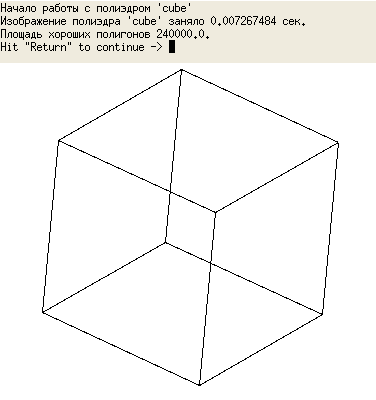
\includegraphics[scale=0.6]{images/222}
\end{center}
\vspace*{-8mm}
\caption{Начало работы с полиэдром куб}\label{fig:term_2}
\end{figure}



\newpage
\begin{thebibliography}{}

\bibitem{wiki-LaTeX}
\link{http://ru.wikipedia.org/wiki/LaTeX}~---
Википедия (свободная энциклопедия) о системе \LaTeX.

\bibitem{texdoc}
\link{http://www.mgena.chat.ru/latex/indru.html}~---
Система \TeX/\LaTeX (конспект).

\bibitem{sources_convex}
\link{http://edu.msiu.ru/files/571-convex.zip}~---
Исходные файлы эталонного проекта <<Выпуклая оболочка>>.
Доступны только при авторизации на образовательном портале МГИУ.

\bibitem{sources_polyedr}
\link{http://edu.msiu.ru/files/1821-polyedr.zip}~---
Исходные файлы эталонного проекта <<Изображение проекции полиэдра>>.
Доступны только при авторизации на образовательном портале МГИУ.

\bibitem{math}
М.Я. Выгодский.
{\em Справочник по высшей математике.}~---
М., АСТ: Астрель, 2008.

\end{thebibliography}

\endinput



\newpage

\end{document}
